\section*{Výsledky měření}
Použili jsme magnetické pole $B_0=\SI{0.4306}{\tesla}$. Pro protony platí $\gamma/2\pi=\SI{42.512990}{\MHz\per\tesla}$ \cite{skripta}.

Předmětem měření byl vodík $^1$H ve vzorku pryže. Larmorova frekvence byla podle \eqref{e:fL} rovna
\begin{equation*}
f_L=\SI{18.306}{\MHz} \,.
\end{equation*}
To se shodovalo s přednastavenou hodnotou na přístroji. Ověřili jsme, že skutečně dochází k resonanci.

Průběh signálu FID při pulzu dlouhém $\tau=\SI{6}{\us}$ a trigrovací dobou $T_0=\SI{400}{\ms}$ je v příloze 1. Průběh pulzu je v příloze 2. Z obrázku vidíme, že v prvních cca \SI{40}{\us} je detektor přesycen a signál je nepoužitelný.
Signál jsme vystředovali přes 10 průběhů (příloha 3) a provedli FFT, abychom dostali NMR spektrum vzorku (příloha 4). 



Z \eqref{e:mz} vyplývá, že amplituda signálu FID by měla být závislá na trigrovací době jako
\begin{equation*}
A(T_0)=A_0(1-exp(-T_0/T_1)) \,,
\end{equation*}
Tato závislost je zanesena do grafu \ref{g:t1} a tabulky \ref{t:t1}.
Fitem jsme určili spin-mřížkovou relaxační dobu
\begin{equation*}
T_1=\SI{65(2)}{\ms} \,,\qquad \qquad A_0 = \num{0.0425(3)} \,.
\end{equation*}
Dále $T_0=\SI{300}{\ms}$.

\begin{graph}[htbp] 
\centering
% GNUPLOT: LaTeX picture with Postscript
\begingroup
  \makeatletter
  \providecommand\color[2][]{%
    \GenericError{(gnuplot) \space\space\space\@spaces}{%
      Package color not loaded in conjunction with
      terminal option `colourtext'%
    }{See the gnuplot documentation for explanation.%
    }{Either use 'blacktext' in gnuplot or load the package
      color.sty in LaTeX.}%
    \renewcommand\color[2][]{}%
  }%
  \providecommand\includegraphics[2][]{%
    \GenericError{(gnuplot) \space\space\space\@spaces}{%
      Package graphicx or graphics not loaded%
    }{See the gnuplot documentation for explanation.%
    }{The gnuplot epslatex terminal needs graphicx.sty or graphics.sty.}%
    \renewcommand\includegraphics[2][]{}%
  }%
  \providecommand\rotatebox[2]{#2}%
  \@ifundefined{ifGPcolor}{%
    \newif\ifGPcolor
    \GPcolorfalse
  }{}%
  \@ifundefined{ifGPblacktext}{%
    \newif\ifGPblacktext
    \GPblacktexttrue
  }{}%
  % define a \g@addto@macro without @ in the name:
  \let\gplgaddtomacro\g@addto@macro
  % define empty templates for all commands taking text:
  \gdef\gplbacktext{}%
  \gdef\gplfronttext{}%
  \makeatother
  \ifGPblacktext
    % no textcolor at all
    \def\colorrgb#1{}%
    \def\colorgray#1{}%
  \else
    % gray or color?
    \ifGPcolor
      \def\colorrgb#1{\color[rgb]{#1}}%
      \def\colorgray#1{\color[gray]{#1}}%
      \expandafter\def\csname LTw\endcsname{\color{white}}%
      \expandafter\def\csname LTb\endcsname{\color{black}}%
      \expandafter\def\csname LTa\endcsname{\color{black}}%
      \expandafter\def\csname LT0\endcsname{\color[rgb]{1,0,0}}%
      \expandafter\def\csname LT1\endcsname{\color[rgb]{0,1,0}}%
      \expandafter\def\csname LT2\endcsname{\color[rgb]{0,0,1}}%
      \expandafter\def\csname LT3\endcsname{\color[rgb]{1,0,1}}%
      \expandafter\def\csname LT4\endcsname{\color[rgb]{0,1,1}}%
      \expandafter\def\csname LT5\endcsname{\color[rgb]{1,1,0}}%
      \expandafter\def\csname LT6\endcsname{\color[rgb]{0,0,0}}%
      \expandafter\def\csname LT7\endcsname{\color[rgb]{1,0.3,0}}%
      \expandafter\def\csname LT8\endcsname{\color[rgb]{0.5,0.5,0.5}}%
    \else
      % gray
      \def\colorrgb#1{\color{black}}%
      \def\colorgray#1{\color[gray]{#1}}%
      \expandafter\def\csname LTw\endcsname{\color{white}}%
      \expandafter\def\csname LTb\endcsname{\color{black}}%
      \expandafter\def\csname LTa\endcsname{\color{black}}%
      \expandafter\def\csname LT0\endcsname{\color{black}}%
      \expandafter\def\csname LT1\endcsname{\color{black}}%
      \expandafter\def\csname LT2\endcsname{\color{black}}%
      \expandafter\def\csname LT3\endcsname{\color{black}}%
      \expandafter\def\csname LT4\endcsname{\color{black}}%
      \expandafter\def\csname LT5\endcsname{\color{black}}%
      \expandafter\def\csname LT6\endcsname{\color{black}}%
      \expandafter\def\csname LT7\endcsname{\color{black}}%
      \expandafter\def\csname LT8\endcsname{\color{black}}%
    \fi
  \fi
  \setlength{\unitlength}{0.0500bp}%
  \begin{picture}(10204.00,6802.00)%
    \gplgaddtomacro\gplbacktext{%
      \csname LTb\endcsname%
      \put(1078,704){\makebox(0,0)[r]{\strut{} 0}}%
      \csname LTb\endcsname%
      \put(1078,1871){\makebox(0,0)[r]{\strut{} 0.01}}%
      \csname LTb\endcsname%
      \put(1078,3037){\makebox(0,0)[r]{\strut{} 0.02}}%
      \csname LTb\endcsname%
      \put(1078,4204){\makebox(0,0)[r]{\strut{} 0.03}}%
      \csname LTb\endcsname%
      \put(1078,5370){\makebox(0,0)[r]{\strut{} 0.04}}%
      \csname LTb\endcsname%
      \put(1078,6537){\makebox(0,0)[r]{\strut{} 0.05}}%
      \csname LTb\endcsname%
      \put(2469,484){\makebox(0,0){\strut{} 10}}%
      \csname LTb\endcsname%
      \put(6100,484){\makebox(0,0){\strut{} 100}}%
      \csname LTb\endcsname%
      \put(9730,484){\makebox(0,0){\strut{} 1000}}%
      \put(176,3620){\rotatebox{-270}{\makebox(0,0){\strut{}$A$}}}%
      \put(5508,154){\makebox(0,0){\strut{}$T_0$ (\si{\ms})}}%
    }%
    \gplgaddtomacro\gplfronttext{%
      \csname LTb\endcsname%
      \put(8820,1097){\makebox(0,0)[r]{\strut{}naměřeno}}%
      \csname LTb\endcsname%
      \put(8820,877){\makebox(0,0)[r]{\strut{}$\num{0.0425}(1-\exp(-x/\num{65.23}))$}}%
    }%
    \gplbacktext
    \put(0,0){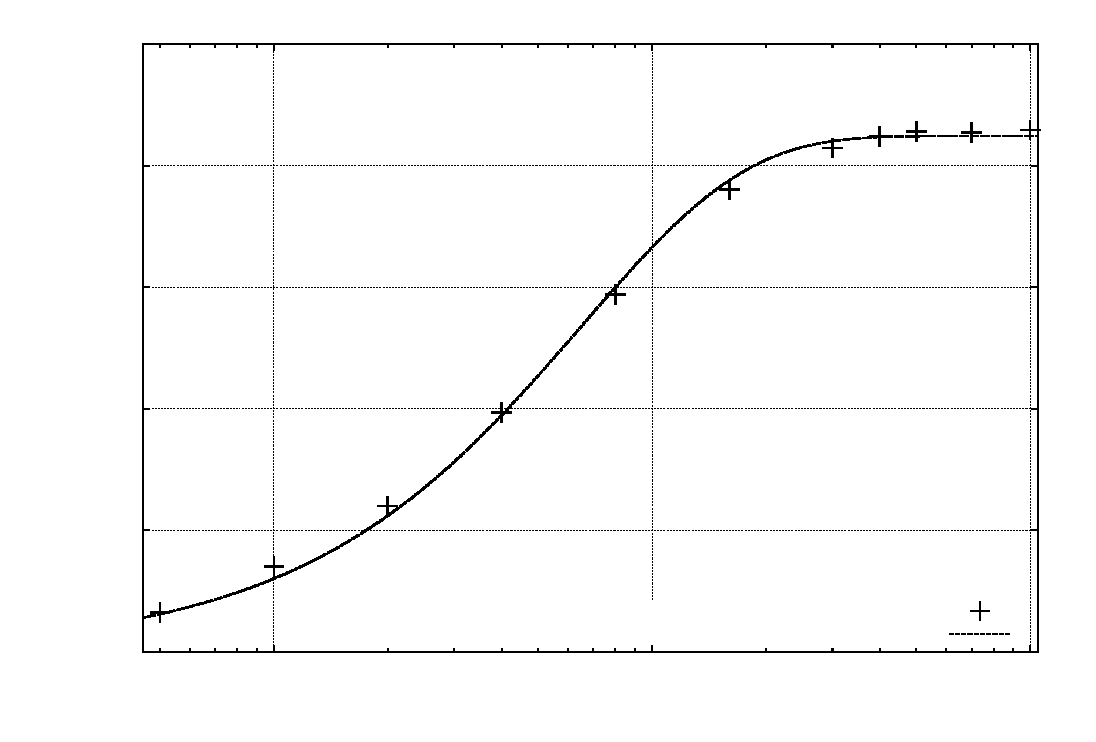
\includegraphics{t1}}%
    \gplfronttext
  \end{picture}%
\endgroup

\caption{Závislost amplitudy signálu FID na trigrovací době $T_0$.}
\label{g:t1}
\end{graph}

\begin{tabulka}[htbp]
\centering
\begin{tabular}{cc|cc}
$T_0$ (\si{\ms}) & $A$ & $T_0$ (\si{\ms}) & $A$ \\\hline
5 & \num{0.00327} & 300 & \num{0.04147} \\
10 & \num{0.00703} & 400 & \num{0.04241} \\
20 & \num{0.01203} & 500 & \num{0.04284} \\
40 & \num{0.01970} & 700 & \num{0.04273} \\
80 & \num{0.02940} & 1000 & \num{0.04296} \\
160 & \num{0.03805} & & \\
\end{tabular}
\caption{Závislost amplitudy signálu FID na trigrovací době $T_0$.}
\label{t:t1}
\end{tabulka}


Dále jsme měřili závislost amplitudy signálu FID na délce pulzu $\tau$. Z \eqref{e:uhel} vyplývá, že závislost by měla mít tvar
\begin{equation*}
A(\tau)=A_1 |\sin(\gamma B_1 \tau) | \,.
\end{equation*}
Tato závislost je vykreslena v grafu \ref{g:tau} a tabulce \ref{t:tau}.
Fitem jsme určili amplitudu pulzního pole
\begin{equation*}
B_1=\SI{1.076(3)}{\milli\tesla}  \,,\qquad \qquad A_1 = \num{0.0408(5)} \,.
\end{equation*}

\begin{graph}[htbp] 
\centering
% GNUPLOT: LaTeX picture with Postscript
\begingroup
  \makeatletter
  \providecommand\color[2][]{%
    \GenericError{(gnuplot) \space\space\space\@spaces}{%
      Package color not loaded in conjunction with
      terminal option `colourtext'%
    }{See the gnuplot documentation for explanation.%
    }{Either use 'blacktext' in gnuplot or load the package
      color.sty in LaTeX.}%
    \renewcommand\color[2][]{}%
  }%
  \providecommand\includegraphics[2][]{%
    \GenericError{(gnuplot) \space\space\space\@spaces}{%
      Package graphicx or graphics not loaded%
    }{See the gnuplot documentation for explanation.%
    }{The gnuplot epslatex terminal needs graphicx.sty or graphics.sty.}%
    \renewcommand\includegraphics[2][]{}%
  }%
  \providecommand\rotatebox[2]{#2}%
  \@ifundefined{ifGPcolor}{%
    \newif\ifGPcolor
    \GPcolorfalse
  }{}%
  \@ifundefined{ifGPblacktext}{%
    \newif\ifGPblacktext
    \GPblacktexttrue
  }{}%
  % define a \g@addto@macro without @ in the name:
  \let\gplgaddtomacro\g@addto@macro
  % define empty templates for all commands taking text:
  \gdef\gplbacktext{}%
  \gdef\gplfronttext{}%
  \makeatother
  \ifGPblacktext
    % no textcolor at all
    \def\colorrgb#1{}%
    \def\colorgray#1{}%
  \else
    % gray or color?
    \ifGPcolor
      \def\colorrgb#1{\color[rgb]{#1}}%
      \def\colorgray#1{\color[gray]{#1}}%
      \expandafter\def\csname LTw\endcsname{\color{white}}%
      \expandafter\def\csname LTb\endcsname{\color{black}}%
      \expandafter\def\csname LTa\endcsname{\color{black}}%
      \expandafter\def\csname LT0\endcsname{\color[rgb]{1,0,0}}%
      \expandafter\def\csname LT1\endcsname{\color[rgb]{0,1,0}}%
      \expandafter\def\csname LT2\endcsname{\color[rgb]{0,0,1}}%
      \expandafter\def\csname LT3\endcsname{\color[rgb]{1,0,1}}%
      \expandafter\def\csname LT4\endcsname{\color[rgb]{0,1,1}}%
      \expandafter\def\csname LT5\endcsname{\color[rgb]{1,1,0}}%
      \expandafter\def\csname LT6\endcsname{\color[rgb]{0,0,0}}%
      \expandafter\def\csname LT7\endcsname{\color[rgb]{1,0.3,0}}%
      \expandafter\def\csname LT8\endcsname{\color[rgb]{0.5,0.5,0.5}}%
    \else
      % gray
      \def\colorrgb#1{\color{black}}%
      \def\colorgray#1{\color[gray]{#1}}%
      \expandafter\def\csname LTw\endcsname{\color{white}}%
      \expandafter\def\csname LTb\endcsname{\color{black}}%
      \expandafter\def\csname LTa\endcsname{\color{black}}%
      \expandafter\def\csname LT0\endcsname{\color{black}}%
      \expandafter\def\csname LT1\endcsname{\color{black}}%
      \expandafter\def\csname LT2\endcsname{\color{black}}%
      \expandafter\def\csname LT3\endcsname{\color{black}}%
      \expandafter\def\csname LT4\endcsname{\color{black}}%
      \expandafter\def\csname LT5\endcsname{\color{black}}%
      \expandafter\def\csname LT6\endcsname{\color{black}}%
      \expandafter\def\csname LT7\endcsname{\color{black}}%
      \expandafter\def\csname LT8\endcsname{\color{black}}%
    \fi
  \fi
  \setlength{\unitlength}{0.0500bp}%
  \begin{picture}(10204.00,6802.00)%
    \gplgaddtomacro\gplbacktext{%
      \csname LTb\endcsname%
      \put(1078,704){\makebox(0,0)[r]{\strut{} 0}}%
      \csname LTb\endcsname%
      \put(1078,1871){\makebox(0,0)[r]{\strut{} 0.01}}%
      \csname LTb\endcsname%
      \put(1078,3037){\makebox(0,0)[r]{\strut{} 0.02}}%
      \csname LTb\endcsname%
      \put(1078,4204){\makebox(0,0)[r]{\strut{} 0.03}}%
      \csname LTb\endcsname%
      \put(1078,5370){\makebox(0,0)[r]{\strut{} 0.04}}%
      \csname LTb\endcsname%
      \put(1078,6537){\makebox(0,0)[r]{\strut{} 0.05}}%
      \csname LTb\endcsname%
      \put(1210,484){\makebox(0,0){\strut{} 0}}%
      \csname LTb\endcsname%
      \put(2210,484){\makebox(0,0){\strut{} 5}}%
      \csname LTb\endcsname%
      \put(3209,484){\makebox(0,0){\strut{} 10}}%
      \csname LTb\endcsname%
      \put(4209,484){\makebox(0,0){\strut{} 15}}%
      \csname LTb\endcsname%
      \put(5209,484){\makebox(0,0){\strut{} 20}}%
      \csname LTb\endcsname%
      \put(6208,484){\makebox(0,0){\strut{} 25}}%
      \csname LTb\endcsname%
      \put(7208,484){\makebox(0,0){\strut{} 30}}%
      \csname LTb\endcsname%
      \put(8208,484){\makebox(0,0){\strut{} 35}}%
      \csname LTb\endcsname%
      \put(9207,484){\makebox(0,0){\strut{} 40}}%
      \put(176,3620){\rotatebox{-270}{\makebox(0,0){\strut{}$A$}}}%
      \put(5508,154){\makebox(0,0){\strut{}$\tau$ (\si{\us})}}%
    }%
    \gplgaddtomacro\gplfronttext{%
      \csname LTb\endcsname%
      \put(4378,6364){\makebox(0,0)[r]{\strut{}naměřeno}}%
      \csname LTb\endcsname%
      \put(4378,6144){\makebox(0,0)[r]{\strut{}$\num{0.0408} |\sin(\num{0.287} \cdot x)|$}}%
    }%
    \gplbacktext
    \put(0,0){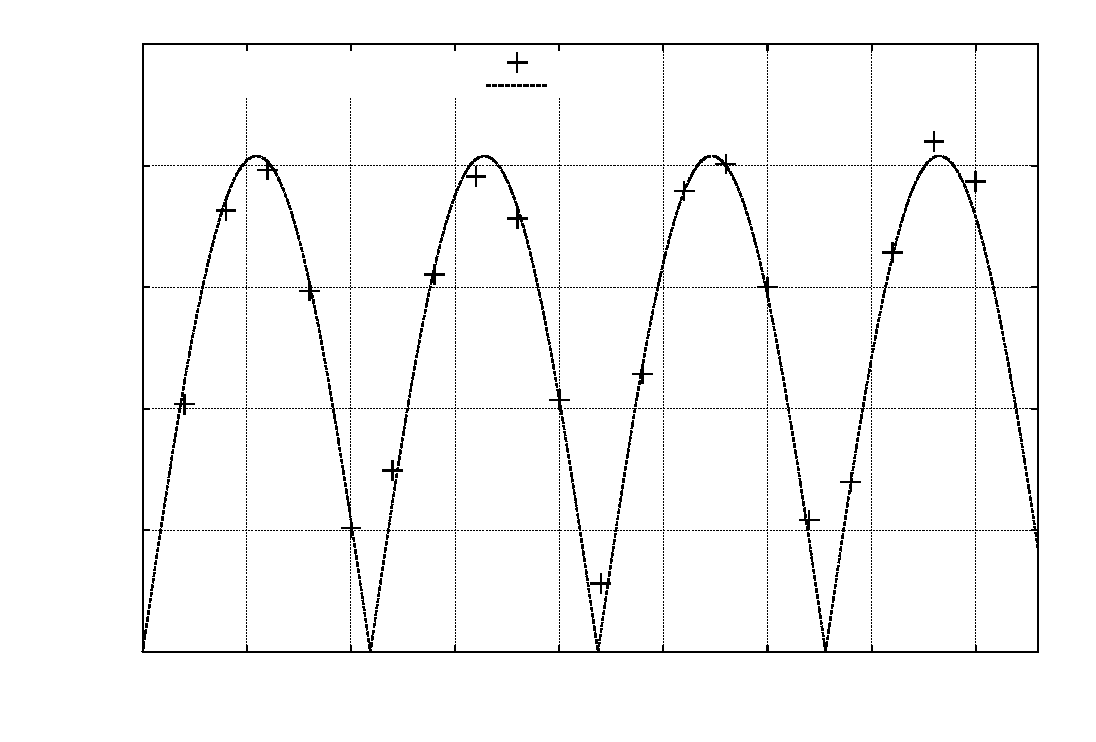
\includegraphics{tau}}%
    \gplfronttext
  \end{picture}%
\endgroup

\caption{Závislost amplitudy signálu FID na délce pulzu $\tau$.}
\label{g:tau}
\end{graph}

\begin{tabulka}[htbp]
\centering
\begin{tabular}{cc|cc|cc}
$\tau$ (\si{\us}) & $A$ & $\tau$ (\si{\us}) & $A$ & $\tau$ (\si{\us}) & $A$ \\\hline
2 & \num{0.02039}  & 16 & \num{0.03913}  & 30 & \num{0.03004}\\
4 & \num{0.03634}  & 18 & \num{0.03568}  & 32 & \num{0.01085}\\
6 & \num{0.03966}  & 20 & \num{0.02075}  & 34 & \num{0.01398}\\
8 & \num{0.02970}  & 20 & \num{0.00563}  & 36 & \num{0.03287}\\
10 & \num{0.01021} & 24 & \num{0.02289}  & 38 & \num{0.04202}\\
12 & \num{0.01496} & 26 & \num{0.03793}  & 40 & \num{0.03872}\\
14 & \num{0.03107} & 28 & \num{0.04015}  & & \\
\end{tabular}
\caption{Závislost amplitudy signálu FID na délce pulzu $\tau$.}
\label{t:tau}
\end{tabulka}

Dále jsme měřili závislost amplitudy signálu spinového echa (viz příloha 5) na odstupu excitačních pulzů $t_{12}$. Z \eqref{e:mt} vyplývá závislost tvaru
\begin{equation*}
A(t_{12})=A_2 \exp(-t_{12}/T_2) \,.
\end{equation*}
Závislost je zanesena do grafu \ref{g:t2} a tabulky \ref{t:t2} (délka prvního pulzu \SI{6}{\us} a druhého \SI{11.7}{\us}).
Fitem jsme určili spin-spinovou relaxační dobu
\begin{equation*}
T_2=\SI{960(40)}{\us}  \,,\qquad \qquad A_2 = \num{0.066(2)} \,.
\end{equation*}
Skutečně platí $T_2 \ll T_1$.


\begin{graph}[htbp] 
\centering
% GNUPLOT: LaTeX picture with Postscript
\begingroup
  \makeatletter
  \providecommand\color[2][]{%
    \GenericError{(gnuplot) \space\space\space\@spaces}{%
      Package color not loaded in conjunction with
      terminal option `colourtext'%
    }{See the gnuplot documentation for explanation.%
    }{Either use 'blacktext' in gnuplot or load the package
      color.sty in LaTeX.}%
    \renewcommand\color[2][]{}%
  }%
  \providecommand\includegraphics[2][]{%
    \GenericError{(gnuplot) \space\space\space\@spaces}{%
      Package graphicx or graphics not loaded%
    }{See the gnuplot documentation for explanation.%
    }{The gnuplot epslatex terminal needs graphicx.sty or graphics.sty.}%
    \renewcommand\includegraphics[2][]{}%
  }%
  \providecommand\rotatebox[2]{#2}%
  \@ifundefined{ifGPcolor}{%
    \newif\ifGPcolor
    \GPcolorfalse
  }{}%
  \@ifundefined{ifGPblacktext}{%
    \newif\ifGPblacktext
    \GPblacktexttrue
  }{}%
  % define a \g@addto@macro without @ in the name:
  \let\gplgaddtomacro\g@addto@macro
  % define empty templates for all commands taking text:
  \gdef\gplbacktext{}%
  \gdef\gplfronttext{}%
  \makeatother
  \ifGPblacktext
    % no textcolor at all
    \def\colorrgb#1{}%
    \def\colorgray#1{}%
  \else
    % gray or color?
    \ifGPcolor
      \def\colorrgb#1{\color[rgb]{#1}}%
      \def\colorgray#1{\color[gray]{#1}}%
      \expandafter\def\csname LTw\endcsname{\color{white}}%
      \expandafter\def\csname LTb\endcsname{\color{black}}%
      \expandafter\def\csname LTa\endcsname{\color{black}}%
      \expandafter\def\csname LT0\endcsname{\color[rgb]{1,0,0}}%
      \expandafter\def\csname LT1\endcsname{\color[rgb]{0,1,0}}%
      \expandafter\def\csname LT2\endcsname{\color[rgb]{0,0,1}}%
      \expandafter\def\csname LT3\endcsname{\color[rgb]{1,0,1}}%
      \expandafter\def\csname LT4\endcsname{\color[rgb]{0,1,1}}%
      \expandafter\def\csname LT5\endcsname{\color[rgb]{1,1,0}}%
      \expandafter\def\csname LT6\endcsname{\color[rgb]{0,0,0}}%
      \expandafter\def\csname LT7\endcsname{\color[rgb]{1,0.3,0}}%
      \expandafter\def\csname LT8\endcsname{\color[rgb]{0.5,0.5,0.5}}%
    \else
      % gray
      \def\colorrgb#1{\color{black}}%
      \def\colorgray#1{\color[gray]{#1}}%
      \expandafter\def\csname LTw\endcsname{\color{white}}%
      \expandafter\def\csname LTb\endcsname{\color{black}}%
      \expandafter\def\csname LTa\endcsname{\color{black}}%
      \expandafter\def\csname LT0\endcsname{\color{black}}%
      \expandafter\def\csname LT1\endcsname{\color{black}}%
      \expandafter\def\csname LT2\endcsname{\color{black}}%
      \expandafter\def\csname LT3\endcsname{\color{black}}%
      \expandafter\def\csname LT4\endcsname{\color{black}}%
      \expandafter\def\csname LT5\endcsname{\color{black}}%
      \expandafter\def\csname LT6\endcsname{\color{black}}%
      \expandafter\def\csname LT7\endcsname{\color{black}}%
      \expandafter\def\csname LT8\endcsname{\color{black}}%
    \fi
  \fi
  \setlength{\unitlength}{0.0500bp}%
  \begin{picture}(10204.00,6802.00)%
    \gplgaddtomacro\gplbacktext{%
      \csname LTb\endcsname%
      \put(1078,1494){\makebox(0,0)[r]{\strut{} 0.01}}%
      \csname LTb\endcsname%
      \put(1078,2335){\makebox(0,0)[r]{\strut{} 0.02}}%
      \csname LTb\endcsname%
      \put(1078,3175){\makebox(0,0)[r]{\strut{} 0.03}}%
      \csname LTb\endcsname%
      \put(1078,4016){\makebox(0,0)[r]{\strut{} 0.04}}%
      \csname LTb\endcsname%
      \put(1078,4856){\makebox(0,0)[r]{\strut{} 0.05}}%
      \csname LTb\endcsname%
      \put(1078,5697){\makebox(0,0)[r]{\strut{} 0.06}}%
      \csname LTb\endcsname%
      \put(1078,6537){\makebox(0,0)[r]{\strut{} 0.07}}%
      \csname LTb\endcsname%
      \put(2266,484){\makebox(0,0){\strut{} 1000}}%
      \csname LTb\endcsname%
      \put(3426,484){\makebox(0,0){\strut{} 2000}}%
      \csname LTb\endcsname%
      \put(4586,484){\makebox(0,0){\strut{} 3000}}%
      \csname LTb\endcsname%
      \put(5746,484){\makebox(0,0){\strut{} 4000}}%
      \csname LTb\endcsname%
      \put(6907,484){\makebox(0,0){\strut{} 5000}}%
      \csname LTb\endcsname%
      \put(8067,484){\makebox(0,0){\strut{} 6000}}%
      \csname LTb\endcsname%
      \put(9227,484){\makebox(0,0){\strut{} 7000}}%
      \put(176,3620){\rotatebox{-270}{\makebox(0,0){\strut{}$A$}}}%
      \put(5508,154){\makebox(0,0){\strut{}$t_{12}$ (\si{\us})}}%
    }%
    \gplgaddtomacro\gplfronttext{%
      \csname LTb\endcsname%
      \put(8820,6364){\makebox(0,0)[r]{\strut{}naměřeno}}%
      \csname LTb\endcsname%
      \put(8820,6144){\makebox(0,0)[r]{\strut{}$\num{0.0665}\exp(-x/\num{957})$}}%
    }%
    \gplbacktext
    \put(0,0){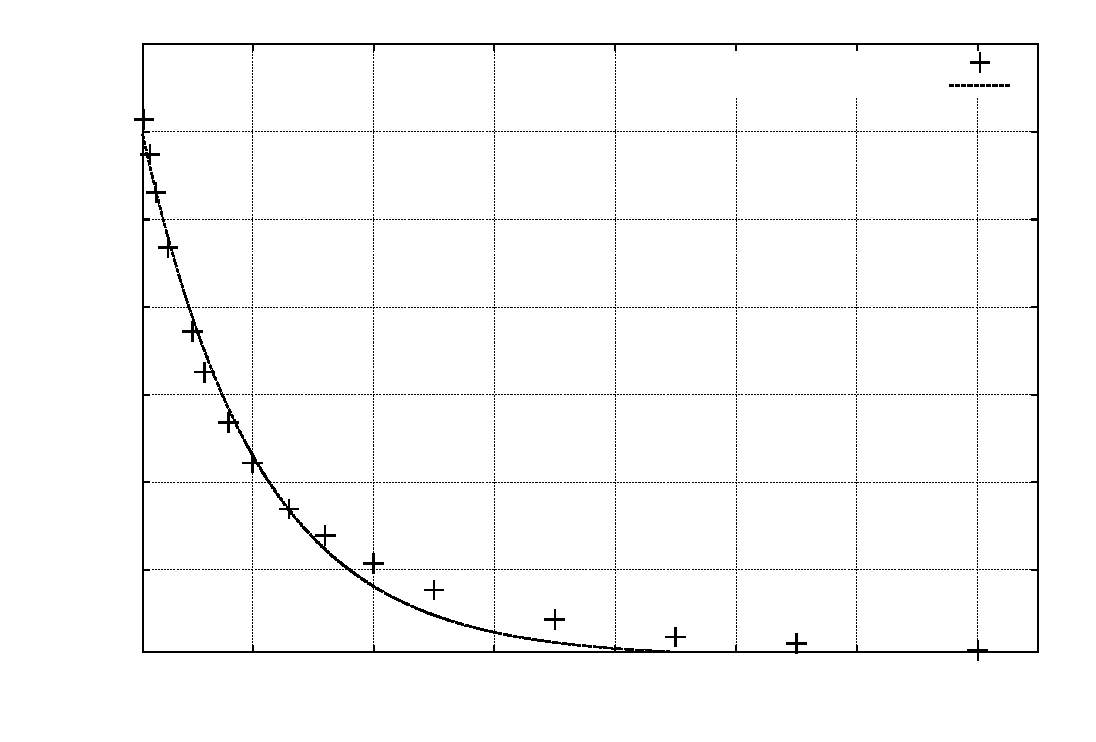
\includegraphics{t2}}%
    \gplfronttext
  \end{picture}%
\endgroup

\caption{Závislost amplitudy signálu spinového echa na odstupu pulzů $t_{12}$.}
\label{g:t2}
\end{graph}

\begin{tabulka}[htbp]
\centering
\begin{tabular}{cc|cc|cc}
$t_{12}$ (\si{\us}) & $A$ & $t_{12}$ (\si{\us}) & $A$ & $t_{12}$ (\si{\us}) & $A$ \\\hline
100 & \num{0.06140}  & 800  & \num{0.02684}  & 3500 & \num{0.00429}\\
150 & \num{0.05743}  & 1000 & \num{0.02220}  & 4500 & \num{0.00230}\\
200 & \num{0.05308}  & 1300 & \num{0.01695}  & 5500 & \num{0.00160}\\
300 & \num{0.04677}  & 1600 & \num{0.01391}  & 7000 & \num{0.00076}\\
500 & \num{0.03721}  & 2000 & \num{0.01068}  &  & \\
600 & \num{0.03256}  & 2500 & \num{0.00769}  &  & \\
\end{tabular}
\caption{Závislost amplitudy signálu spinového echa na odstupu pulzů $t_{12}$.}
\label{t:t2}
\end{tabulka}




Vyšetřili jsme závislost standardní odchylky šumového napětí na počtu sumací, výsledky jsou v grafu \ref{g:s} a tabulce \ref{t:s}. V grafu \ref{g:sum} je zakresleno několik spekter pro vybrané počty sumací (jsou vertikálně posunuté pro lepší porovnatelnost). Podle očekávání se intenzita šumu snižuje.

\begin{graph}[htbp] 
\centering
% GNUPLOT: LaTeX picture with Postscript
\begingroup
  \makeatletter
  \providecommand\color[2][]{%
    \GenericError{(gnuplot) \space\space\space\@spaces}{%
      Package color not loaded in conjunction with
      terminal option `colourtext'%
    }{See the gnuplot documentation for explanation.%
    }{Either use 'blacktext' in gnuplot or load the package
      color.sty in LaTeX.}%
    \renewcommand\color[2][]{}%
  }%
  \providecommand\includegraphics[2][]{%
    \GenericError{(gnuplot) \space\space\space\@spaces}{%
      Package graphicx or graphics not loaded%
    }{See the gnuplot documentation for explanation.%
    }{The gnuplot epslatex terminal needs graphicx.sty or graphics.sty.}%
    \renewcommand\includegraphics[2][]{}%
  }%
  \providecommand\rotatebox[2]{#2}%
  \@ifundefined{ifGPcolor}{%
    \newif\ifGPcolor
    \GPcolorfalse
  }{}%
  \@ifundefined{ifGPblacktext}{%
    \newif\ifGPblacktext
    \GPblacktexttrue
  }{}%
  % define a \g@addto@macro without @ in the name:
  \let\gplgaddtomacro\g@addto@macro
  % define empty templates for all commands taking text:
  \gdef\gplbacktext{}%
  \gdef\gplfronttext{}%
  \makeatother
  \ifGPblacktext
    % no textcolor at all
    \def\colorrgb#1{}%
    \def\colorgray#1{}%
  \else
    % gray or color?
    \ifGPcolor
      \def\colorrgb#1{\color[rgb]{#1}}%
      \def\colorgray#1{\color[gray]{#1}}%
      \expandafter\def\csname LTw\endcsname{\color{white}}%
      \expandafter\def\csname LTb\endcsname{\color{black}}%
      \expandafter\def\csname LTa\endcsname{\color{black}}%
      \expandafter\def\csname LT0\endcsname{\color[rgb]{1,0,0}}%
      \expandafter\def\csname LT1\endcsname{\color[rgb]{0,1,0}}%
      \expandafter\def\csname LT2\endcsname{\color[rgb]{0,0,1}}%
      \expandafter\def\csname LT3\endcsname{\color[rgb]{1,0,1}}%
      \expandafter\def\csname LT4\endcsname{\color[rgb]{0,1,1}}%
      \expandafter\def\csname LT5\endcsname{\color[rgb]{1,1,0}}%
      \expandafter\def\csname LT6\endcsname{\color[rgb]{0,0,0}}%
      \expandafter\def\csname LT7\endcsname{\color[rgb]{1,0.3,0}}%
      \expandafter\def\csname LT8\endcsname{\color[rgb]{0.5,0.5,0.5}}%
    \else
      % gray
      \def\colorrgb#1{\color{black}}%
      \def\colorgray#1{\color[gray]{#1}}%
      \expandafter\def\csname LTw\endcsname{\color{white}}%
      \expandafter\def\csname LTb\endcsname{\color{black}}%
      \expandafter\def\csname LTa\endcsname{\color{black}}%
      \expandafter\def\csname LT0\endcsname{\color{black}}%
      \expandafter\def\csname LT1\endcsname{\color{black}}%
      \expandafter\def\csname LT2\endcsname{\color{black}}%
      \expandafter\def\csname LT3\endcsname{\color{black}}%
      \expandafter\def\csname LT4\endcsname{\color{black}}%
      \expandafter\def\csname LT5\endcsname{\color{black}}%
      \expandafter\def\csname LT6\endcsname{\color{black}}%
      \expandafter\def\csname LT7\endcsname{\color{black}}%
      \expandafter\def\csname LT8\endcsname{\color{black}}%
    \fi
  \fi
  \setlength{\unitlength}{0.0500bp}%
  \begin{picture}(9070.00,5668.00)%
    \gplgaddtomacro\gplbacktext{%
      \csname LTb\endcsname%
      \put(1342,704){\makebox(0,0)[r]{\strut{} 0}}%
      \csname LTb\endcsname%
      \put(1342,1487){\makebox(0,0)[r]{\strut{} 0.0001}}%
      \csname LTb\endcsname%
      \put(1342,2270){\makebox(0,0)[r]{\strut{} 0.0002}}%
      \csname LTb\endcsname%
      \put(1342,3054){\makebox(0,0)[r]{\strut{} 0.0003}}%
      \csname LTb\endcsname%
      \put(1342,3837){\makebox(0,0)[r]{\strut{} 0.0004}}%
      \csname LTb\endcsname%
      \put(1342,4620){\makebox(0,0)[r]{\strut{} 0.0005}}%
      \csname LTb\endcsname%
      \put(1342,5403){\makebox(0,0)[r]{\strut{} 0.0006}}%
      \csname LTb\endcsname%
      \put(1474,484){\makebox(0,0){\strut{} 0}}%
      \csname LTb\endcsname%
      \put(2374,484){\makebox(0,0){\strut{} 0.1}}%
      \csname LTb\endcsname%
      \put(3274,484){\makebox(0,0){\strut{} 0.2}}%
      \csname LTb\endcsname%
      \put(4174,484){\makebox(0,0){\strut{} 0.3}}%
      \csname LTb\endcsname%
      \put(5074,484){\makebox(0,0){\strut{} 0.4}}%
      \csname LTb\endcsname%
      \put(5973,484){\makebox(0,0){\strut{} 0.5}}%
      \csname LTb\endcsname%
      \put(6873,484){\makebox(0,0){\strut{} 0.6}}%
      \csname LTb\endcsname%
      \put(7773,484){\makebox(0,0){\strut{} 0.7}}%
      \csname LTb\endcsname%
      \put(8673,484){\makebox(0,0){\strut{} 0.8}}%
      \put(176,3053){\rotatebox{-270}{\makebox(0,0){\strut{}$\sigma^2_{\bar{u^n}}$ ($\cdot 10^{-4}$)}}}%
      \put(5073,154){\makebox(0,0){\strut{}$1/\sqrt{N}$}}%
    }%
    \gplgaddtomacro\gplfronttext{%
      \csname LTb\endcsname%
      \put(3190,5230){\makebox(0,0)[r]{\strut{}naměřeno}}%
      \csname LTb\endcsname%
      \put(3190,5010){\makebox(0,0)[r]{\strut{}$\num{0.000691}/\sqrt{N}$}}%
    }%
    \gplbacktext
    \put(0,0){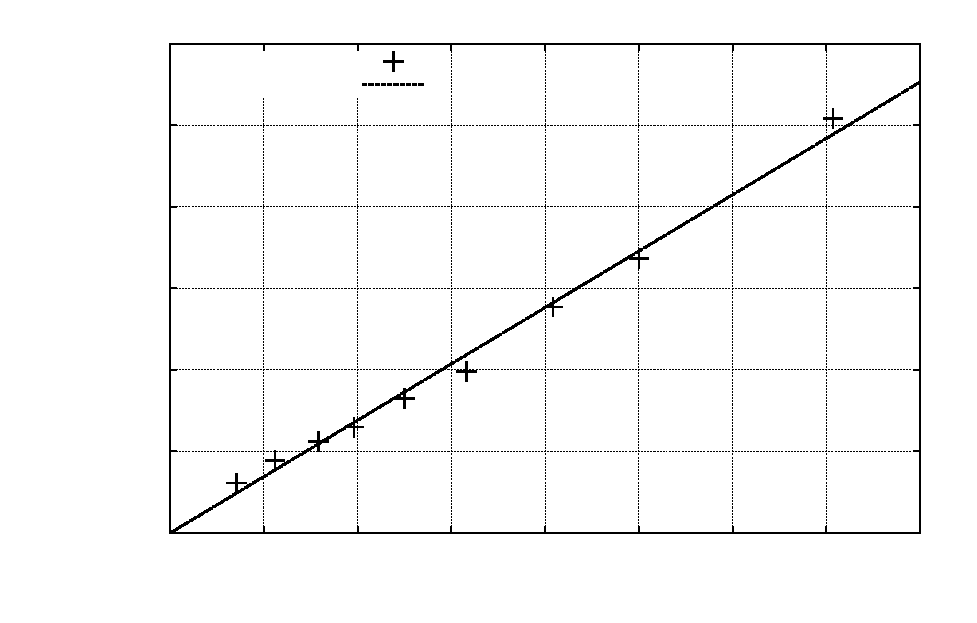
\includegraphics{s}}%
    \gplfronttext
  \end{picture}%
\endgroup

\caption{Závislost standardní odchylky šumového napětí na počtu sumací}
\label{g:s}
\end{graph}

\begin{tabulka}[htbp]
\centering
\begin{tabular}{cc}
$N$ & $\sigma^2_{\bar{u^n}}$ ($\cdot 10^{-4}$) \\\hline
2  & 5,079 \\
4 & 3,363 \\
6 & 2,772 \\
10 & 1,978 \\
16 & 1,651 \\
26 & 1,297 \\
40 & 1,119 \\
80 & 0,8890 \\
200 & 0,6124 \\
\end{tabular}
\caption{Závislost standardní odchylky šumového napětí na počtu sumací}
\label{t:s}
\end{tabulka}

\begin{graph}[htbp] 
\centering
% GNUPLOT: LaTeX picture with Postscript
\begingroup
  \makeatletter
  \providecommand\color[2][]{%
    \GenericError{(gnuplot) \space\space\space\@spaces}{%
      Package color not loaded in conjunction with
      terminal option `colourtext'%
    }{See the gnuplot documentation for explanation.%
    }{Either use 'blacktext' in gnuplot or load the package
      color.sty in LaTeX.}%
    \renewcommand\color[2][]{}%
  }%
  \providecommand\includegraphics[2][]{%
    \GenericError{(gnuplot) \space\space\space\@spaces}{%
      Package graphicx or graphics not loaded%
    }{See the gnuplot documentation for explanation.%
    }{The gnuplot epslatex terminal needs graphicx.sty or graphics.sty.}%
    \renewcommand\includegraphics[2][]{}%
  }%
  \providecommand\rotatebox[2]{#2}%
  \@ifundefined{ifGPcolor}{%
    \newif\ifGPcolor
    \GPcolortrue
  }{}%
  \@ifundefined{ifGPblacktext}{%
    \newif\ifGPblacktext
    \GPblacktextfalse
  }{}%
  % define a \g@addto@macro without @ in the name:
  \let\gplgaddtomacro\g@addto@macro
  % define empty templates for all commands taking text:
  \gdef\gplbacktext{}%
  \gdef\gplfronttext{}%
  \makeatother
  \ifGPblacktext
    % no textcolor at all
    \def\colorrgb#1{}%
    \def\colorgray#1{}%
  \else
    % gray or color?
    \ifGPcolor
      \def\colorrgb#1{\color[rgb]{#1}}%
      \def\colorgray#1{\color[gray]{#1}}%
      \expandafter\def\csname LTw\endcsname{\color{white}}%
      \expandafter\def\csname LTb\endcsname{\color{black}}%
      \expandafter\def\csname LTa\endcsname{\color{black}}%
      \expandafter\def\csname LT0\endcsname{\color[rgb]{1,0,0}}%
      \expandafter\def\csname LT1\endcsname{\color[rgb]{0,1,0}}%
      \expandafter\def\csname LT2\endcsname{\color[rgb]{0,0,1}}%
      \expandafter\def\csname LT3\endcsname{\color[rgb]{1,0,1}}%
      \expandafter\def\csname LT4\endcsname{\color[rgb]{0,1,1}}%
      \expandafter\def\csname LT5\endcsname{\color[rgb]{1,1,0}}%
      \expandafter\def\csname LT6\endcsname{\color[rgb]{0,0,0}}%
      \expandafter\def\csname LT7\endcsname{\color[rgb]{1,0.3,0}}%
      \expandafter\def\csname LT8\endcsname{\color[rgb]{0.5,0.5,0.5}}%
    \else
      % gray
      \def\colorrgb#1{\color{black}}%
      \def\colorgray#1{\color[gray]{#1}}%
      \expandafter\def\csname LTw\endcsname{\color{white}}%
      \expandafter\def\csname LTb\endcsname{\color{black}}%
      \expandafter\def\csname LTa\endcsname{\color{black}}%
      \expandafter\def\csname LT0\endcsname{\color{black}}%
      \expandafter\def\csname LT1\endcsname{\color{black}}%
      \expandafter\def\csname LT2\endcsname{\color{black}}%
      \expandafter\def\csname LT3\endcsname{\color{black}}%
      \expandafter\def\csname LT4\endcsname{\color{black}}%
      \expandafter\def\csname LT5\endcsname{\color{black}}%
      \expandafter\def\csname LT6\endcsname{\color{black}}%
      \expandafter\def\csname LT7\endcsname{\color{black}}%
      \expandafter\def\csname LT8\endcsname{\color{black}}%
    \fi
  \fi
  \setlength{\unitlength}{0.0500bp}%
  \begin{picture}(10204.00,7936.00)%
    \gplgaddtomacro\gplbacktext{%
      \csname LTb\endcsname%
      \put(198,704){\makebox(0,0)[r]{\strut{}}}%
      \csname LTb\endcsname%
      \put(198,2312){\makebox(0,0)[r]{\strut{}}}%
      \csname LTb\endcsname%
      \put(198,3920){\makebox(0,0)[r]{\strut{}}}%
      \csname LTb\endcsname%
      \put(198,5527){\makebox(0,0)[r]{\strut{}}}%
      \csname LTb\endcsname%
      \put(198,7135){\makebox(0,0)[r]{\strut{}}}%
      \csname LTb\endcsname%
      \put(330,484){\makebox(0,0){\strut{}-80}}%
      \csname LTb\endcsname%
      \put(922,484){\makebox(0,0){\strut{}-70}}%
      \csname LTb\endcsname%
      \put(1515,484){\makebox(0,0){\strut{}-60}}%
      \csname LTb\endcsname%
      \put(2107,484){\makebox(0,0){\strut{}-50}}%
      \csname LTb\endcsname%
      \put(2699,484){\makebox(0,0){\strut{}-40}}%
      \csname LTb\endcsname%
      \put(3292,484){\makebox(0,0){\strut{}-30}}%
      \csname LTb\endcsname%
      \put(3884,484){\makebox(0,0){\strut{}-20}}%
      \csname LTb\endcsname%
      \put(4476,484){\makebox(0,0){\strut{}-10}}%
      \csname LTb\endcsname%
      \put(5069,484){\makebox(0,0){\strut{} 0}}%
      \csname LTb\endcsname%
      \put(5661,484){\makebox(0,0){\strut{} 10}}%
      \csname LTb\endcsname%
      \put(6253,484){\makebox(0,0){\strut{} 20}}%
      \csname LTb\endcsname%
      \put(6845,484){\makebox(0,0){\strut{} 30}}%
      \csname LTb\endcsname%
      \put(7438,484){\makebox(0,0){\strut{} 40}}%
      \csname LTb\endcsname%
      \put(8030,484){\makebox(0,0){\strut{} 50}}%
      \csname LTb\endcsname%
      \put(8622,484){\makebox(0,0){\strut{} 60}}%
      \csname LTb\endcsname%
      \put(9215,484){\makebox(0,0){\strut{} 70}}%
      \csname LTb\endcsname%
      \put(9807,484){\makebox(0,0){\strut{} 80}}%
      \put(176,4187){\rotatebox{-270}{\makebox(0,0){\strut{}}}}%
      \put(5068,154){\makebox(0,0){\strut{}frekvence (\si{\kHz})}}%
    }%
    \gplgaddtomacro\gplfronttext{%
      \csname LTb\endcsname%
      \put(858,7498){\makebox(0,0)[r]{\strut{}200}}%
      \csname LTb\endcsname%
      \put(858,7278){\makebox(0,0)[r]{\strut{}26}}%
      \csname LTb\endcsname%
      \put(858,7058){\makebox(0,0)[r]{\strut{}6}}%
      \csname LTb\endcsname%
      \put(858,6838){\makebox(0,0)[r]{\strut{}2}}%
    }%
    \gplbacktext
    \put(0,0){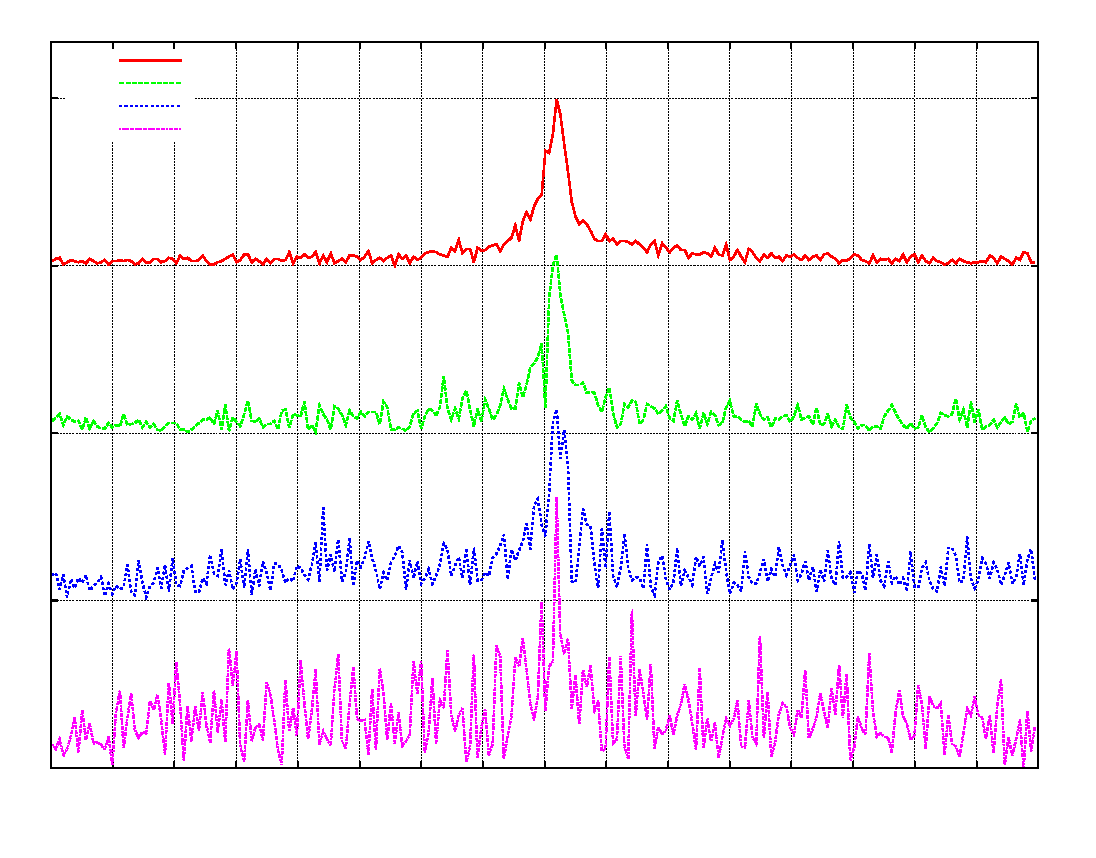
\includegraphics{sum}}%
    \gplfronttext
  \end{picture}%
\endgroup

\caption{Spektrum pro vybrané počty sumací.}
\label{g:sum}
\end{graph}